\documentclass[a4paper,oneside,12pt]{extreport}

\usepackage{mmap}
\usepackage[T2A]{fontenc}
\usepackage[utf8]{inputenc}
\usepackage[english,russian]{babel}


% Текст отчёта следует печатать, соблюдая следующие размеры полей:
% левое — 30 мм, правое — 15 мм, верхнее и нижнее — 20 мм.
\usepackage[left=20mm, right=15mm, top=15mm, bottom=15mm]{geometry}

% \setlength{\parindent}{1.25cm} % Абзацный отступ

\usepackage{setspace}
%\onehalfspacing % Полуторный интервал

\frenchspacing % Равномерные пробелы
\usepackage{indentfirst} % Красная строка

\usepackage{microtype}
\sloppy

\usepackage{titlesec}
\titlespacing*{\chapter}{0pt}{-30pt}{8pt}
\titlespacing*{\section}{\parindent}{*4}{*4}
\titlespacing*{\subsection}{\parindent}{*4}{*4}
\titleformat{\chapter}{\LARGE\bfseries}{\thechapter}{20pt}{\LARGE\bfseries}
\titleformat{\section}{\Large\bfseries}{\thesection}{40pt}{\Large\bfseries}

\usepackage{graphicx}
\usepackage{caption}

\usepackage[unicode,pdftex]{hyperref}
\hypersetup{hidelinks}

%% title begin
\usepackage{wrapfig}

\makeatletter
	\def\vhrulefill#1{\leavevmode\leaders\hrule\@height#1\hfill \kern\z@}
\makeatother
%% title end

%% begin code
\usepackage{listings}
\usepackage{xcolor}

\lstset{
	basicstyle=\footnotesize\ttfamily,
	breakatwhitespace=true,
	breaklines=true,
	commentstyle=\color{gray},
	frame=single,
	keywordstyle=\color{blue},
	stringstyle=\color{red},
	tabsize=8
}

\lstdefinestyle{lispinline}{
	frame=none,
	language=Lisp
}

\newcommand{\code}[1]{\texttt{#1}}
%% end code

%% begin theorem
\usepackage{amsthm}

\makeatletter
\newtheoremstyle{indented}
	{}% measure of space to leave above the theorem
	{}% measure of space to leave below the theorem
	{}% name of font to use in the body of the theorem
	{\parindent}% measure of space to indent
	{\bfseries}% name of head font
	{.}% punctuation between head and body
	{ }% space after theorem head; " " = normal interword space
	{}% header specification (empty for default)
\makeatother

\theoremstyle{indented}

\newtheorem{definition}{Определение}[section]
\newtheorem{example}{Пример}[section]
\newtheorem{theorem}{Теорема}[section]
\newtheorem{task}{Задание}

\makeatletter
\DeclareRobustCommand\bfseriesitshape{%
	\not@math@alphabet\itshapebfseries\relax
	\fontseries\bfdefault
	\fontshape\itdefault
	\selectfont
}
\makeatother

\DeclareTextFontCommand{\textbfit}{\bfseriesitshape}
\DeclareTextFontCommand{\define}{\bfseriesitshape}
%% end theorem

%% begin columns
\usepackage{etoolbox,refcount}
\usepackage{multicol}

\newcounter{countitems}
\newcounter{nextitemizecount}
\newcommand{\setupcountitems}{%
	\stepcounter{nextitemizecount}%
	\setcounter{countitems}{0}%
	\preto\item{\stepcounter{countitems}}%
}
\makeatletter
\newcommand{\computecountitems}{%
	\edef\@currentlabel{\number\c@countitems}%
	\label{countitems@\number\numexpr\value{nextitemizecount}-1\relax}%
}
\newcommand{\nextitemizecount}{%
	\getrefnumber{countitems@\number\c@nextitemizecount}%
}
\newcommand{\previtemizecount}{%
	\getrefnumber{countitems@\number\numexpr\value{nextitemizecount}-1\relax}%
}
\makeatother
\newenvironment{AutoMultiColItemize}{%
	\ifnumcomp{\nextitemizecount}{>}{3}{\begin{multicols}{2}}{}%
		\setupcountitems\begin{itemize}}%
		{\end{itemize}%
		\unskip\computecountitems\ifnumcomp{\previtemizecount}{>}{3}{\end{multicols}}{}}
\makeatother
\newenvironment{AutoMultiColEnumerate}{%
	\ifnumcomp{\nextitemizecount}{>}{3}{\begin{multicols}{2}}{}%
		\setupcountitems\begin{enumerate}}%
		{\end{enumerate}%
		\unskip\computecountitems\ifnumcomp{\previtemizecount}{>}{3}{\end{multicols}}{}}
%% end columns



\begin{document}

\begin{titlepage}
	{\large % 14pt instead of 12pt
	\onehalfspacing
	\centering

	\begin{wrapfigure}[7]{l}{0.14\linewidth}
		\vspace{3mm}
		\hspace{-10mm}
		
\includegraphics[width=\linewidth]{img/b_logo}
		% \includegraphics[width=0.93\linewidth]{inc/img/bmstu-logo}
	\end{wrapfigure}
	{\singlespacing \footnotesize \bfseries Министерство науки и высшего образования Российской Федерации\\Федеральное государственное бюджетное образовательное учреждение\\высшего образования\\<<Московский государственный технический университет\\имени Н.~Э.~Баумана\\ (национальный исследовательский университет)>>\\(МГТУ им. Н.~Э.~Баумана)\\}

	\vspace{-2.2mm}
	\vhrulefill{0.9mm}\\
	\vspace{-7.5mm}
	\vhrulefill{0.2mm}\\
	\vspace{2mm}

	{\doublespacing \small \raggedright ФАКУЛЬТЕТ \hspace{5mm} \underline{«Информатика и системы управления»}\\
	КАФЕДРА \hspace{10mm} \underline{«Программное обеспечение ЭВМ и информационные технологии»}\\}

	\vspace{20mm}

	\begin{center}
		\noindent\begin{minipage}{1.2\textwidth}\centering
			\textbf{ОТЧЕТ ПО ЛАБОРАТОРНОЙ РАБОТЕ №6}\newline
			\textbf{По курсу: "Операционные системы"}\newline\newline\newline
		\end{minipage}
	\end{center}

	\vspace{20mm}

	\noindent ~~Тема \underline{~~~~~~~~~~~~~~~~~~~~~~~~~~~Системный вызов open()~~~~~~~~~~~~~~~~~~~~~~~~~~~~~~~~~~~}\newline
	\noindent ~~Группа \underline{~~~~~~~~~~~~~~~~~~~~~~~~~~~~~~~~~~ИУ7-63Б~~~~~~~~~~~~~~~~~~~~~~~~~~~~~~~~~~~~~~~~~~~~~~~~~}\newline
	\noindent ~~Студент \underline{~~~~~~~~~~~~~~~~~~~~~~~~~~~Сукочева А.~~~~~~~~~~~~~~~~~~~~~~~~~~~~~~~~~~~~~~~~~~~~~~~~~~}\newline
	\noindent ~~Преподаватель \underline{~~~~~~~~~~~~~~~~~~~Рязанова Н.Ю.~~~~~~~~~~~~~~~~~~~~~~~~~~~~~~~~~~~~~~~~~~~~~}\newline


	\begin{center}
		\vfill
		Москва~---~\the\year
		~г.
	\end{center}
	}



\end{titlepage}

\setcounter{page}{2}

\section*{Практическая часть}

\begin{task}
    Первая программа.
    \begin{lstlisting}[language=C]
#include <stdio.h>
#include <fcntl.h>

#define OK 0
#define FILE_NAME "alphabet.txt"
#define BUFF_SIZE 20

#define GREEN "\33[32m"
#define BLUE "\33[34m"
#define RED "\33[31m"

int main()
{
    int fd = open(FILE_NAME, O_RDONLY); 

    FILE *fs1 = fdopen(fd, "r");
    char buff1[BUFF_SIZE];
    setvbuf(fs1, buff1, _IOFBF, BUFF_SIZE); 

    FILE *fs2 = fdopen(fd, "r");
    char buff2[BUFF_SIZE];
    setvbuf(fs2, buff2, _IOFBF, BUFF_SIZE);

    int flag1 = 1, flag2 = 2;

    while (flag1 == 1 || flag2 == 1)
    {
        char c;
        flag1 = fscanf(fs1, "%c", &c);
        if (flag1 == 1)
        {
            fprintf(stdout, GREEN "%c", c);
        }
        flag2 = fscanf(fs2, "%c", &c);
        if (flag2 == 1)
        {
            fprintf(stdout, BLUE "%c", c);
        }
    }

    return OK;
}
    \end{lstlisting}

    \newpage

    \begin{center}
        \textbf{Анализ}        
    \end{center}

    Данная программа считывает информацию из файла 'alphabet.txt', который содержит строку символов 'Abcdefghijklmnopqrstuvwxyz'.
    И при помощи двух буферов посимвольно выводит считанные символы в стандартный поток вывода stdout.  

    Зеленым цветом показан вывод при помощи первого буфера, синим при помощи второго буфера.
    
    % При первом вызове fscanf первый буфер заполняется полностью, т.е. 20 символами.
    % После  
    В файле '/usr/include/x86\_64-linux-gnu/bits/types/FILE.h' было создано дополнительное 
    имя для структуры FILE, которая используется в нашей программе.
    \begin{lstlisting}[language=C]
        typedef struct _IO_FILE FILE;
    \end{lstlisting}

    В файле 'cat /usr/include/x86\_64-linux-gnu/bits/libio.h' находится описание структуры \_IO\_FILE
    \begin{lstlisting}[language=C]
struct _IO_FILE
{
    int _flags; /* High-order word is _IO_MAGIC; rest is flags. */
#define _IO_file_flags _flags

    /* The following pointers correspond to the C++ streambuf protocol. */
    /* Note:  Tk uses the _IO_read_ptr and _IO_read_end fields directly. */
    char *_IO_read_ptr;   /* Current read pointer */
    char *_IO_read_end;   /* End of get area. */
    char *_IO_read_base;  /* Start of putback+get area. */
    char *_IO_write_base; /* Start of put area. */
    char *_IO_write_ptr;  /* Current put pointer. */
    char *_IO_write_end;  /* End of put area. */
    char *_IO_buf_base;   /* Start of reserve area. */
    char *_IO_buf_end;    /* End of reserve area. */
    /* The following fields are used to support backing up and undo. */
    char *_IO_save_base;   /* Pointer to start of non-current get area. */
    char *_IO_backup_base; /* Pointer to first valid character of backup area */
    char *_IO_save_end;    /* Pointer to end of non-current get area. */

    struct _IO_marker *_markers;

    struct _IO_FILE *_chain;

    int _fileno;
#if 0
    int _blksize;
#else
    int _flags2;
#endif
    _IO_off_t _old_offset; /* This used to be _offset but it's too small.  */

#define __HAVE_COLUMN /* temporary */
    /* 1+column number of pbase(); 0 is unknown. */
    unsigned short _cur_column;
    signed char _vtable_offset;
    char _shortbuf[1];

    /*  char* _save_gptr;  char* _save_egptr; */

    _IO_lock_t *_lock;
#ifdef _IO_USE_OLD_IO_FILE
};
    \end{lstlisting}

    \newpage
    \begin{figure}[ht!]
        \centering{
            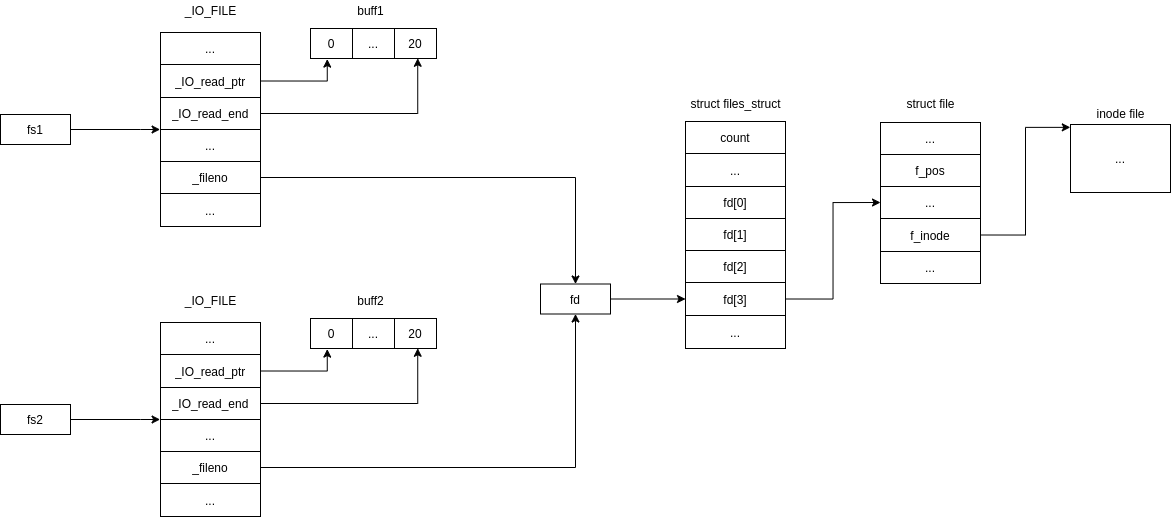
\includegraphics[width=1\textwidth]{img/Diagram_1.png}
            \caption{Связь между дескрипторами в первой программе}}
    \end{figure}
    

    В начале функции main open() создает новый файловый дескриптор для открытого
    только на чтение (O\_RDONLY) файла 'alphabet.txt', запись в системной таблице открытых файлов. 
    Эта запись регистрирует смещение в файле и флаги состояния файла.
    
    Далее fdopen() создает два указателя на структуру FILE, приведенную выше.
    В данных структурах поле \_fileno будет содержать дескриптор, который вернула
    функция fopen(). Для fs1 и fs2 эти поля будут равны 3.
    % (наименьший дескриптор, который еще не открыт). 

    Функция setvbuf() изменяет тип буферизации для fs1 и fs2 на
    полную буферизацию, а также явно задает размер буфера 20 байт.

    Далее при первом вызове fscanf() буфер fs1 заполнится полностью, 
    т.е. первыми 20 символами. 
    Значение f\_pos в структуре struct\_file открытого файла увеличится на 20.
    Далее при первом вызове fscanf() для fs2 в buff2 считаются оставшиеся 6 символов,
    начиная с f\_pos (т.к. fs1 и fs2 ссылаются на один и тот же дескриптор fd).

    Далее в цикле поочередно выводятся символы из buff1 и buff2.
    Т.к. в buff2 записались оставшиеся 6 символов, после 6 итерации
    цикла будут выводится символы только из buff1.

    \begin{figure}[ht!]
        \centering{
            
\includegraphics[width=0.8\textwidth]{img/res_1.png}
            \caption{Результат работы первой программы}}
    \end{figure}

\end{task}

\newpage

\begin{task}
    Вторая программа. Один поток.
    \begin{lstlisting}[language=C]
        //testKernelIO.c
#include <fcntl.h>
#include <unistd.h> // read, write.

#define OK 0
#define FILE_NAME "alphabet.txt"

int main()
{
	char c;

	int fd1 = open(FILE_NAME, O_RDONLY);
	int fd2 = open(FILE_NAME, O_RDONLY);

	while (read(fd1, &c, 1) && read(fd2, &c, 1))
	{
		write(1, &c, 1);
		write(1, &c, 1);
	}

	write(1, "\n", 1);
	return OK;
}
    \end{lstlisting}

    
    
    \begin{figure}[ht!]
        \centering{
            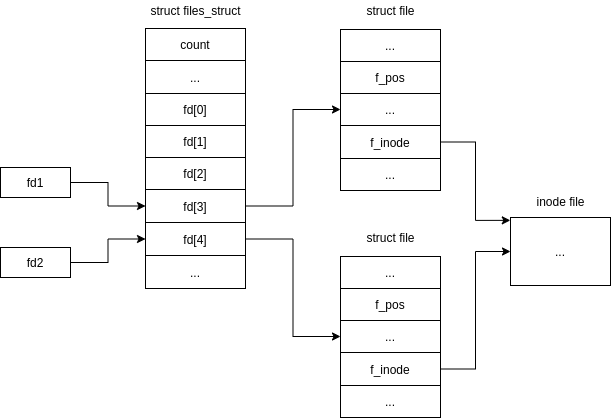
\includegraphics[width=0.8\textwidth]{img/Diagram_2.png}
            \caption{Связь между дескрипторами во второй программе}}
    \end{figure}
    
    \newpage
    \begin{center}
        \textbf{Анализ}        
    \end{center}

    В данной программе создается два файловых дескриптора при помощи функции open(). 
    При этом создается две разные структуры struct\_file, описывающие файл.
    Далее в цикле поочередно считываются символы из файла и выводятся на экран.
    Т.к. созданы две структуры struct file, то у каждой структуры будет
    свой f\_pos и смещения в файловых дескрипторах будут независимы,
    поэтому на экран будут дважды выводится символы одного и того же файла.

    \begin{figure}[ht!]
        \centering{
            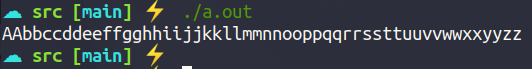
\includegraphics[width=0.8\textwidth]{img/res_2.png}
            \caption{Результат работы второй программы}}
    \end{figure}
    % В системной таблице открытых файлов создаются две новые записи, дескрипторы 

    Вторая программа. Два потока.
    \begin{lstlisting}[language=C]
#include <fcntl.h>
#include <unistd.h> // read, write.
#include <pthread.h>
#include <stdio.h>

#define OK 0
#define ERROR_THREAD_CREATE -1
#define FILE_NAME "alphabet.txt"

void read_file(int fd)
{
    char c;
    while (read(fd, &c, 1))
    {
        write(1, &c, 1);
    }
}

void *thr_fn(void *arg)
{
    int fd = open(FILE_NAME, O_RDONLY);
    read_file(fd);
}

int main()
{
    pthread_t tid;

    int fd = open(FILE_NAME, O_RDONLY);

    int err = pthread_create(&tid, NULL, thr_fn, 0);
    if (err)
    {
        return ERROR_THREAD_CREATE;
    }

    read_file(fd);
    pthread_join(tid, NULL);

    return OK;
}
    \end{lstlisting}

    В программе также, как и при реализации с одним потоком, создается
    два файловых дескриптора для открытого файла, записи в системной таблице открытых файлов.
    У каждой записи будет свое смещение f\_pos.
    Т.к. главный поток ждет окончания дочернего, то гарантируется вывод
    всего алфавита дважды.
    Порядок, в котором будут выводится символы алфавита, неизвестен,
    т.к. вывод производится параллельно.


    \begin{figure}[ht!]
        \centering{
            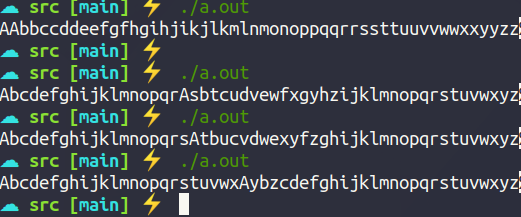
\includegraphics[width=0.8\textwidth]{img/res_2_pthread.png}
            \caption{Результат работы второй программы при двух потоках}}
    \end{figure}

\end{task}

\begin{task}
    Третья программа. Один поток.

    \begin{lstlisting}[language=C]
#include <stdio.h>
#include <sys/stat.h>

#define FILE_NAME "task3.txt"
#define OK 0

void Info()
{
    struct stat statbuf;

    stat(FILE_NAME, &statbuf);
    printf("inode: %ld\n", statbuf.st_ino);
    printf("st_size: %ld\n", statbuf.st_size);
    printf("st_blksize: %ld\n\n", statbuf.st_blksize);
}

int main()
{

    FILE *f1 = fopen(FILE_NAME, "w");
    Info();

    FILE *f2 = fopen(FILE_NAME, "w");
    Info();

    char c = 'a'; // 97
    while (c <= 'z')
    {
        if (c % 2)
        {
            fprintf(f1, "%c", c); // acej...
        }
        else
        {
            fprintf(f2, "%c", c); // bdfh...
        }
        c++;
    }

    fclose(f1);
    Info();

    fclose(f2);
    Info();

    return OK;
}
    \end{lstlisting}

    В данной программе файл 'task3.txt' открывается 2 раза для записи.
    Выполняется ввод через стандартную библиотеку С (stdio.h). 
    fprintf() - буферизованный ввод/вывод. 
    Буфер создается без нашего явного вмешательства.
    Сначала информация пишется в буфер, а из буфера информация 
    переписывается в файл в результате 3-ех действий:
    \begin{enumerate}
        \item буфер полон;
        \item принудительная запись fflush();
        \item если вызван fclose().
    \end{enumerate}   

    \begin{figure}[ht!]
        \centering{
            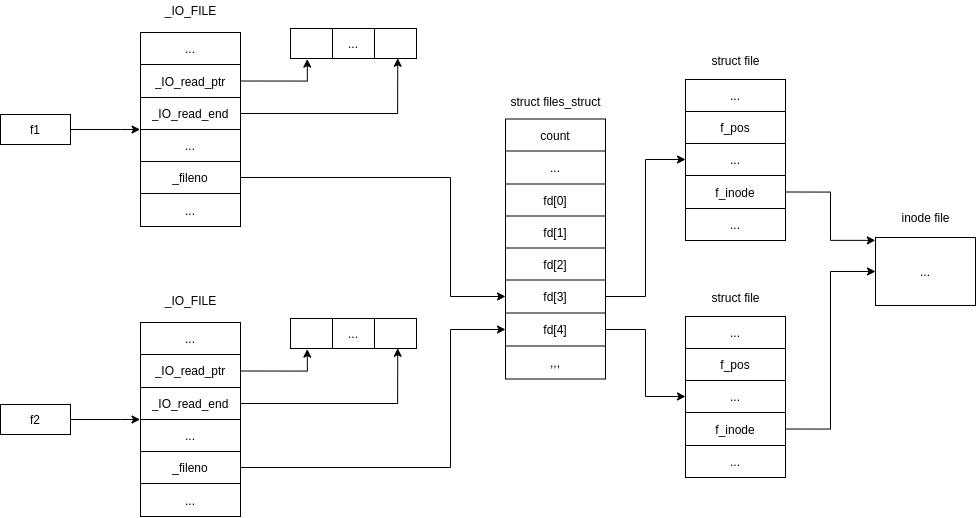
\includegraphics[width=1\textwidth]{img/Diagram_3.png}
            \caption{Связь между дескрипторами в третьей программе}}
    \end{figure}

    В нашей программе символы, имеющие нечетный код в таблице ASCII
    записываются в буфер, который находится в дескрипторе f1, 
    в f2 соответственно записываются четные. 
    Таким образом в буфере, который содержится в f1 будут символы: 'acej...', 
    а в f2 'bdfh...'.
    В нашем случае информация из фубера запишется в файл при вызове fclose().
    Т.к. f\_pos независимы у каждого дескриптора файла, то при закрытии файла
    запись будет производиться начиная с начала файла в обоих случаях.
    Таким образом информация, которая будет записана в файл, после первого вызова
    fclose() будет потеряна в результате второго вызова fclose() рис. \ref{ref:res31}.   
   
    \begin{figure}[ht!]
        \centering{
            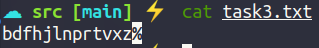
\includegraphics[width=0.7\textwidth]{img/res_3_1.png}
            \caption{Результат работы третьей программы }
            \label{ref:res31}}
    \end{figure}

    Если поменять вызовы fclose() местами, то будет потеряна информация,
    которая содержится во втором буфере рис. \ref{ref:res32}.
    \begin{lstlisting}[language=C]
    fclose(f2);
    fclose(f1);
    \end{lstlisting}

    \begin{figure}[ht!]
        \centering{
            
\includegraphics[width=0.7\textwidth]{img/res_3_2.png}
            \caption{Результат работы третьей программы с другим порядком вызовов fclose()}
            \label{ref:res32}}
    \end{figure}

    \newpage
    С помощью stat после каждого вызова fopen() и fclose()
    показана некоторая информация о файле рис. \ref{ref:info}. 

    \begin{figure}[ht!]
        \centering{
            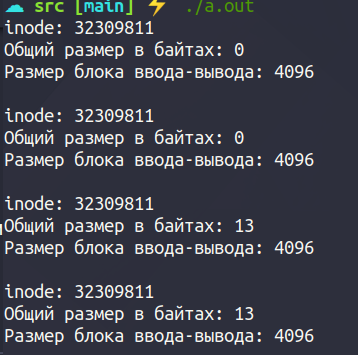
\includegraphics[width=0.7\textwidth]{img/info_3.png}
            \caption{Информация, полученная при помощи stat}
            \label{ref:info}}
    \end{figure}

    \begin{figure}[ht!]
        \centering{
            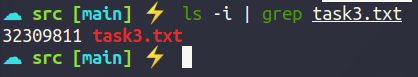
\includegraphics[width=0.7\textwidth]{img/inod.png}
            \caption{inode файла task3.txt}
            \label{ref:info}}
    \end{figure}

    \newpage

    Третья программа. Два потока.
    \begin{lstlisting}[language=C]
#include <stdio.h>
#include <sys/stat.h>
#include <pthread.h>

#define FILE_NAME "task3_pthread.txt"
#define ERROR_THREAD_CREATE -1
#define OK 0

void Info()
{
    struct stat statbuf;

    stat(FILE_NAME, &statbuf);
    printf("inode: %ld\n", statbuf.st_ino);
    printf("st_size: %ld\n", statbuf.st_size);
    printf("st_blksize: %ld\n\n", statbuf.st_blksize);
}

void WriteToFile(char c)
{
    FILE *f = fopen(FILE_NAME, "w");
    Info();

    while (c <= 'z')
    {
        fprintf(f, "%c", c);
        c += 2;
    }

    fclose(f);
    Info();
}

void *thr_fn(void *arg)
{
    WriteToFile('b');
}

int main()
{
    pthread_t tid;

    int err = pthread_create(&tid, NULL, thr_fn, NULL);
    if (err)
    {
        return ERROR_THREAD_CREATE;
    }

    WriteToFile('a');
    pthread_join(tid, NULL);

    return OK;
}
    \end{lstlisting}

    В данной программе создается поток.
    Главный поток записывает в файл символы, начиная с 'a', в то время, как созданный
    нами поток записывает символы, начиная с 'b'. 
    Так же как и в приведенной выше программе с одним потоком происходит потеря данных.
    Данные будут записаны из того буфера (который содержится в дескрипторе), для которого
    будет вызван fclose() последним, потому что он перезапишет данные с начала файла.
    Можно принудительно в главном потоке вызвать sleep(), чтобы в файле были данные 
    записанные из главного потока. Тогда результат работы представлен на рис. \ref{ref:res32}.
    
    \begin{lstlisting}[language=C]
        sleep(1);
        WriteToFile('a');
    \end{lstlisting}

\end{task}

\section*{Заключение}

В ходе выполнения данной лабораторной работы были проанализированы три программы.
Открытие файла при помощи open() создает новый файловый дескриптор для открытого 
файла, запись в системной таблице открытых файлов.
У различных дескрипторов открытого файла смещения не зависят друг от друга.
Поэтому чтобы избежать потери данных необходимо учитывать, что файл может быть открыт 
несколько раз.

\end{document}